\documentclass[a4paper]{article}

%% Language and font encodings
\usepackage[english]{babel}
\usepackage[utf8x]{inputenc}
\usepackage[T1]{fontenc}

%% Sets page size and margins
\usepackage[a4paper,top=3cm,bottom=2cm,left=3cm,right=3cm,marginparwidth=1.75cm]{geometry}

%% Useful packages
\usepackage{amsmath}
\usepackage{graphicx}
\usepackage{textpos}
\usepackage{float}
\usepackage[colorinlistoftodos]{todonotes}
\usepackage[colorlinks=true, allcolors=black]{hyperref}
\usepackage[numbered,framed]{matlab-prettifier}
\usepackage{relsize}
\usepackage{amsmath}
\usepackage{amssymb}
\usepackage{amsthm}

%% Package for graphs
\usepackage{tikz}

%% Package for loading MatLab
\usepackage[framed,numbered,autolinebreaks,useliterate]{mcode}

\setlength{\parindent}{0pt}
\newcommand{\p}{\mathbb{P}}

\title{\vspace*{2cm}17.7 Graph Planarity\vspace*{-1.5cm}}
\date{}

\begin{document}
\maketitle

\begin{textblock*}{100mm}(0cm,-5.5cm)
\Huge 17.7
\end{textblock*}

\section*{Graph Drawing}
\subsection*{Question 1}
Script tutte.m (pg.\pageref{Ptutte}) is a function which accepts as input a graph and cycle and outputs a planar drawing of the graph using Tutte's Theorem. Then Q1.m (pg.\pageref{PQ1}) is a script which applies tutte.m to a graph and cycle specified by the user. Figure \ref{fig:Q1a} includes drawings generated of the five platonic solids via this script.

\begin{figure}
    \centering
    \includegraphics[width=0.48\columnwidth]{Platonic_4.png}
    \includegraphics[width=0.48\columnwidth]{Platonic_6.png}
    \includegraphics[width=0.48\columnwidth]{Platonic_8.png}
    \includegraphics[width=0.48\columnwidth]{Platonic_12.png}
    \includegraphics[width=0.48\columnwidth]{Platonic_20.png}
    \caption{Planar drawings of the platonic solids generated by Tutte's algorithm with script tutte.m}
    \label{fig:Q1a}
\end{figure}

\vspace{\baselineskip}
Specifying $K_2 + P_5$ via an edge list (pg.\pageref{K2_P5}) we can then applying Tutte's Theorem as above. Figure \ref{fig:Q1b} includes the output.

\begin{figure}[H]
    \centering
    \includegraphics[width=0.55\columnwidth]{K2_P5.png}
    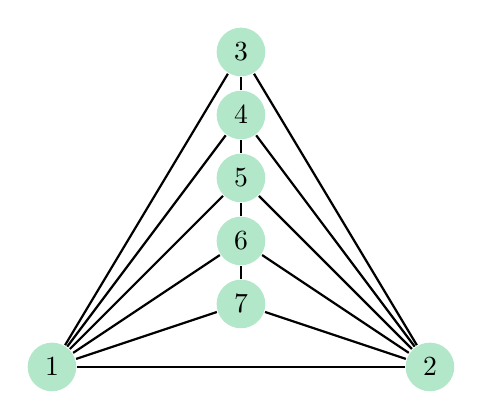
\begin{tikzpicture}
        [scale=.8,auto=left,thick,every node/.style={circle,fill=blue!30!green!30}]
        \node (1) at (-3,0) {1};
        \node (2) at ( 3,0) {2};
        \node (3) at ( 0,5) {3};
        \node (4) at ( 0,4) {4};
        \node (5) at ( 0,3) {5};
        \node (6) at ( 0,2) {6};
        \node (7) at ( 0,1) {7};
        
        \path [-] (1) edge (2);
        
        \path [-] (3) edge (4);
        \path [-] (4) edge (5);
        \path [-] (5) edge (6);
        \path [-] (6) edge (7);
        
        \path [-] (1) edge (3);
        \path [-] (1) edge (4);
        \path [-] (1) edge (5);
        \path [-] (1) edge (6);
        \path [-] (1) edge (7);
        \path [-] (2) edge (3);
        \path [-] (2) edge (4);
        \path [-] (2) edge (5);
        \path [-] (2) edge (6);
        \path [-] (2) edge (7);
    \end{tikzpicture}
    \caption{Planar drawing of $K_2 + P_5$. Left: graph generated with tutte.m and edge list K2\_P5.txt (pg.\pageref{K2_P5}). Right: diagram with distorted spacing to make clearer the relative positioning of the vertices.}
    \label{fig:Q1b}
\end{figure}


\section*{Bridges \& Components}

\subsection*{Question 2}
Script find\_comp.m (pg.\pageref{Pfind_comp}) accepts a graph in the form of an adjacency list and determines the graphs components in the form of vertex lists. Combining these with the original graph then the edge list for each component can also be found. In addition, accepting an adjacency list leaves space for application of this method, without adaption, to finding weakly connected components of directed graphs. Both these points are utilised in script find\_bridges.m (pg.\pageref{Pfind_bridges}) to find the bridges of a given cycle. Each bridge is specified as an edge list and is returned together with its vertices of attachment.

\section*{Interleaving}

\subsection*{Question 3}

Suppose $G$ is a graph with a cycle $C$ that has $l$ bridges $B_1, ..., B_l$. Let $C[i,...,j]$ denote the subgraph with edges $E(C) \cup B_i \cup \hdots \cup B_j$. $G$ is planar if and only if the following condition is met:
\begin{center}
    $C[i]$ is planar for $1 \leq i \leq l$ and the interleave graph $H$ is bipartite.
\end{center}

To understand this result let us consider the following observations.

\vspace{\baselineskip}
\textbf{First observation:} we observe the simple result that a planar graph can have no non-planar subgraphs. If you draw a graph in the plane then you have also successfully drawn all its subgraphs in the plane as well and they are all therefore planar too.

\vspace{\baselineskip}
\textbf{Second observation:} we observe that for two interleaving bridges, $B_1$ and $B_2$, with graphs $C[1]$ and $C[2]$ both planar then $C[1,2]$ is also planar but it can be drawn in the plane if and only if $B_1$ and $B_2$ are on opposite sides of the cycle. For example consider the simple graph included in figure \ref{fig:Q3a}. However, if two graphs don't interleave then they can easily be drawn on the same side of the cycle - consider figure \ref{fig:Q3b}.

\vspace{\baselineskip}
We now prove the desired result as follows:

\vspace{\baselineskip}
\textbf{$\Leftarrow$ direction:} Given $G$ planar by our first observation we have all subgraphs planar and so $C[i]$ is planar for $1 \leq i \leq l$. G is planar so consider a drawing of G, by our second observation we note that no two bridges drawn on the same side of the cycle can be interleaved. This means we can divide the bridges into two sets which within themselves have no two bridges interleaved, in other words we can make a bipartite interleave graph.

\vspace{\baselineskip}
\textbf{$\Rightarrow$ direction:} Given the condition above, by our second observation we can successfully draw $G$ by always placing interleaving bridges on opposite sides of the cycle. We will be able to do this because the interleave graph $H$ is bipartite. Therefore $G$ is planar.

\begin{figure}[H]
    \centering
    \begin{minipage}{0.48\textwidth}
        \centering
        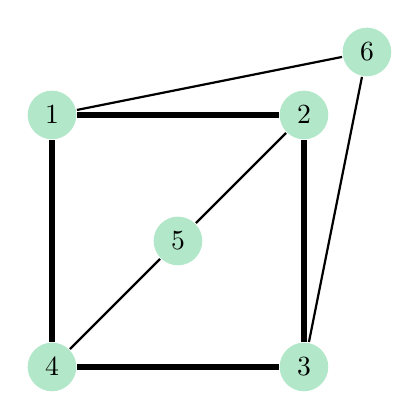
\begin{tikzpicture}
            [scale=.8,auto=left,thick,every node/.style={circle,fill=blue!30!green!30}]
            \node (1) at (0,4) {1};
            \node (2) at (4,4) {2};
            \node (3) at (4,0) {3};
            \node (4) at (0,0) {4};
            \node (5) at (2,2) {5};
            \node (6) at (5,5) {6};
            % the cycle
            \draw[line width=2pt] (1) -- (2);
            \draw[line width=2pt] (2) -- (3);
            \draw[line width=2pt] (3) -- (4);
            \draw[line width=2pt] (4) -- (1);
            % bridges
            \draw (5) -- (2);
            \draw (5) -- (4);
            \draw (6) -- (1);
            \draw (6) -- (3);
        \end{tikzpicture}
    \end{minipage}\hfill
    \begin{minipage}{0.48\textwidth}
        \centering
        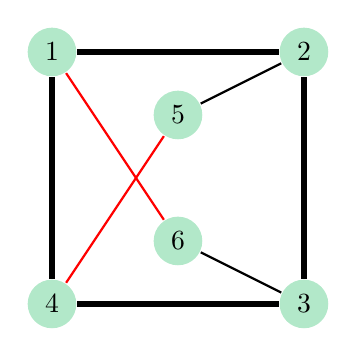
\begin{tikzpicture}
            [scale=.8,auto=left,thick,every node/.style={circle,fill=blue!30!green!30}]
            \node (1) at (0,4) {1};
            \node (2) at (4,4) {2};
            \node (3) at (4,0) {3};
            \node (4) at (0,0) {4};
            \node (5) at (2,3) {5};
            \node (6) at (2,1) {6};
            % the cycle
            \draw[line width=2pt] (1) -- (2);
            \draw[line width=2pt] (2) -- (3);
            \draw[line width=2pt] (3) -- (4);
            \draw[line width=2pt] (4) -- (1);
            % bridges
            \draw (5) -- (2);
            \draw[red] (5) -- (4);
            \draw[red] (6) -- (1);
            \draw (6) -- (3);
        \end{tikzpicture}
    \end{minipage}
    \caption{To preserve planarity two interleaving bridges must be drawn on opposite sides of the cycle}
    \label{fig:Q3a}
\end{figure}

\begin{figure}[H]
    \centering
    \begin{minipage}{0.48\textwidth}
        \centering
        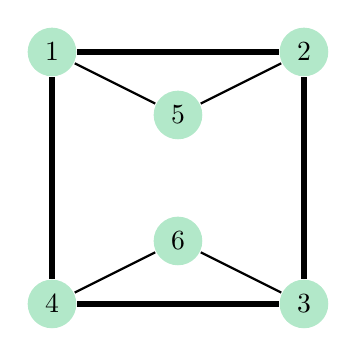
\begin{tikzpicture}
            [scale=.8,auto=left,thick,every node/.style={circle,fill=blue!30!green!30}]
            \node (1) at (0,4) {1};
            \node (2) at (4,4) {2};
            \node (3) at (4,0) {3};
            \node (4) at (0,0) {4};
            \node (5) at (2,3) {5};
            \node (6) at (2,1) {6};
            % the cycle
            \draw[line width=2pt] (1) -- (2);
            \draw[line width=2pt] (2) -- (3);
            \draw[line width=2pt] (3) -- (4);
            \draw[line width=2pt] (4) -- (1);
            % bridges
            \draw (5) -- (1);
            \draw (5) -- (2);
            \draw (6) -- (3);
            \draw (6) -- (4);
        \end{tikzpicture}
    \end{minipage}\hfill
    \begin{minipage}{0.48\textwidth}
        \centering
        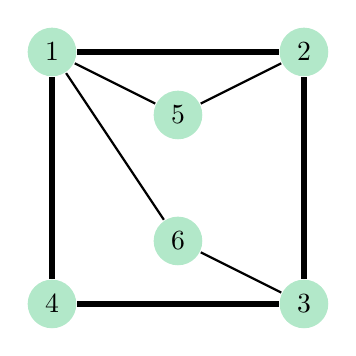
\begin{tikzpicture}
            [scale=.8,auto=left,thick,every node/.style={circle,fill=blue!30!green!30}]
            \node (1) at (0,4) {1};
            \node (2) at (4,4) {2};
            \node (3) at (4,0) {3};
            \node (4) at (0,0) {4};
            \node (5) at (2,3) {5};
            \node (6) at (2,1) {6};
            % the cycle
            \draw[line width=2pt] (1) -- (2);
            \draw[line width=2pt] (2) -- (3);
            \draw[line width=2pt] (3) -- (4);
            \draw[line width=2pt] (4) -- (1);
            % bridges
            \draw (5) -- (1);
            \draw (5) -- (2);
            \draw (6) -- (1);
            \draw (6) -- (3);
        \end{tikzpicture}
    \end{minipage}
    \caption{Two non-interleaving bridges can easily be drawn on the same side of the cycle without compromising planarity}
    \label{fig:Q3b}
\end{figure}

\subsection*{Question 4}

Script find\_interleave.m (pg.\pageref{Pfind_interleave}) constructs the interleave graph from a cycle and its bridges. It does this by comparing each pair of bridges in turn to test if they interleave. Script is\_bipartite.m (pg.\pageref{Pis_bipartite}) determines if a graph is bipartite by colouring vertices one of two colours until either a contradiction arises or the vertex set is fully partitioned. Figure \ref{fig:Q4} includes an example of a 5-cycle with three simple bridges (chords). The script correctly identifies the corresponding interleave graph.

\begin{figure}[H]
    \centering
    \begin{minipage}{0.65\textwidth}
        \centering
        \begin{verbatim}
>> cycle = [1,2,3,4,5];
>> bridges = {[1,3],[1,3];[2,4],[2,4];[3,5],[3,5];};
>> find_interleave(cycle, bridges)

ans =

     1     2
     2     3
        \end{verbatim}
    \end{minipage}\hfill
    \begin{minipage}{0.35\textwidth}
        \centering
        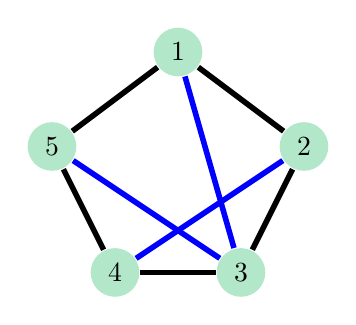
\begin{tikzpicture}
            [scale=.8,auto=left,thick,every node/.style={circle,fill=blue!30!green!30}]
            \node (1) at (0, 3.5) {1};
            \node (2) at (2, 2) {2};
            \node (3) at (1, 0) {3};
            \node (4) at (-1, 0) {4};
            \node (5) at (-2,2) {5};
            \draw[line width=2pt] (1) -- (2);
            \draw[line width=2pt] (2) -- (3);
            \draw[line width=2pt] (3) -- (4);
            \draw[line width=2pt] (4) -- (5);
            \draw[line width=2pt] (5) -- (1);
            \draw[line width=2pt, blue] (1) -- (3);
            \draw[line width=2pt, blue] (2) -- (4);
            \draw[line width=2pt, blue] (3) -- (5);

        \end{tikzpicture}
    \end{minipage}
    \caption{An example application of find\_interleave.m}
    \label{fig:Q4}
\end{figure}

\section*{The Core of a Graph}

\subsection*{Question 5}

Script find\_core.m (pg.\pageref{Pfind_core}) constructs the core $G^*$ of a graph $G$. Figure \ref{fig:Q5code} includes example application of this function to graphs $G_1$ and $G_2$ which are drawn in figure \ref{fig:Q5}. The script correctly determines the core of $G_1$ to be the empty graph and the core of $G_2$ to be itself.

\begin{figure}[H]
    \centering
    \begin{minipage}{0.48\textwidth}
        \centering
        \begin{verbatim}
>> edges1 = [1,2;2,3;3,4;4,1;1,3]

edges1 =

     1     2
     2     3
     3     4
     4     1
     1     3

>> find_core(edges1)

ans =

  0×2 empty double matrix
  
  
  
  
  
  
        \end{verbatim}
    \end{minipage}\hfill
    \begin{minipage}{0.48\textwidth}
        \centering
        \begin{verbatim}
>> edges2 = [1,2;2,3;3,4;4,1;1,3;2,4]

edges2 =

     1     2
     2     3
     3     4
     4     1
     1     3
     2     4

>> find_core(edges2)

ans =

     1     2
     2     3
     3     4
     4     1
     1     3
     2     4
        \end{verbatim}
    \end{minipage}
    \caption{Output from running find\_core.m in the command window on graphs $G_1$ and $G_2$ which are drawn in figure \ref{fig:Q5}.}
    \label{fig:Q5code}
\end{figure}

\begin{figure}[H]
    \centering
    \begin{minipage}{0.48\textwidth}
        \centering
        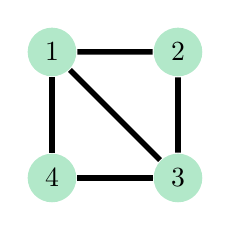
\begin{tikzpicture}
            [scale=.8,auto=left,thick,every node/.style={circle,fill=blue!30!green!30}]
            \node (1) at (0,2) {1};
            \node (2) at (2,2) {2};
            \node (3) at (2,0) {3};
            \node (4) at (0,0) {4};
            % the cycle
            \draw[line width=2pt] (1) -- (2);
            \draw[line width=2pt] (2) -- (3);
            \draw[line width=2pt] (3) -- (4);
            \draw[line width=2pt] (4) -- (1);
            \draw[line width=2pt] (1) -- (3);
        \end{tikzpicture}
    \end{minipage}\hfill
    \begin{minipage}{0.48\textwidth}
        \centering
        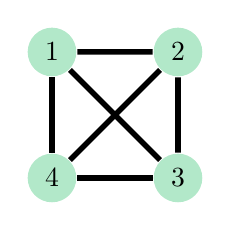
\begin{tikzpicture}
            [scale=.8,auto=left,thick,every node/.style={circle,fill=blue!30!green!30}]
            \node (1) at (0,2) {1};
            \node (2) at (2,2) {2};
            \node (3) at (2,0) {3};
            \node (4) at (0,0) {4};
            % the cycle
            \draw[line width=2pt] (1) -- (2);
            \draw[line width=2pt] (2) -- (3);
            \draw[line width=2pt] (3) -- (4);
            \draw[line width=2pt] (4) -- (1);
            \draw[line width=2pt] (1) -- (3);
            \draw[line width=2pt] (2) -- (4);
        \end{tikzpicture}
    \end{minipage}
    \caption{Drawings of graphs $G_1$ and $G_2$ on the left and right respectively.}
    \label{fig:Q5}
\end{figure}

\subsection*{Question 6}

\subsubsection*{Procedure for finding a cycle in a finite graph of minimum degree 2}
Choose any vertex to start. Carry out a walk as follows:
\begin{itemize}
    \item
    Inspect the neighbourhood (all adjacent vertices) of the current vertex.
    \begin{itemize}
        \item 
        If the neighbourhood contains a previously visited vertex then move to that vertex to form a cycle. The cycle will include all edges traversed since first visiting that vertex.
        \item
        Otherwise all neighbours are unvisited. Choose any neighbour to move to and then repeat the process.
    \end{itemize}
\end{itemize}
Since the graph is minimum degree at least 2 this means that the procedure will never fail because every vertex will have at least one vertex to travel to next, excluding the one visited immediately previously. Furthermore, the procedure will terminate because the graph is finite - by the pigeon-hole principle after $v(G)$ steps the next step must encounter a visited vertex and so form a cycle.

\subsubsection*{Procedure for finding a cycle with a chord in a graph of minimum degree at least 3}
Choose any vertex to start. Carry out a walk as follows:
\begin{itemize}
    \item
    Inspect the neighbourhood (all adjacent vertices) of the current vertex $u$.
    \begin{itemize}
        \item
        If the neighbourhood contains at least one unvisited vertex then choose one and move to that vertex and return to the first step.
        \item
        Otherwise all neighbours are visited. Given that the graph is of minimum degree at least 3 then there will be at least 2 previously visited vertices (excluding the vertex visited immediately previously). Choose two of these vertices, say $v_1$ and $v_2$. As in the previous procedure, returning to these vertices will form cycles, without loss of generality let $v_1$ form the larger cycle. We observe that the edge $uv_2$ forms of a chord to the cycle formed by $v_1$. Terminate the procedure.
    \end{itemize}
\end{itemize}
Since the graph is finite the procedure will definitely terminate. Similarly to the first procedure, this procedure can take a most $v(G)$ before the next step must terminate the process. Figure \ref{fig:Q6} includes an example to visualise this procedure.

Script find\_cycle\_with\_chord.m (pg.\pageref{Pfind_cycle_with_chord}) implements this procedure to find a cycle with a chord in a graph of minimum degree 3. Noting that by construction a core $G^*$ contains no vertices of degree 1 or 2 we have that this script will find a cycle with a chord in a non-empty core $G^*$.

\begin{figure}[H]
    \centering
    \begin{minipage}{0.48\textwidth}
        \centering
        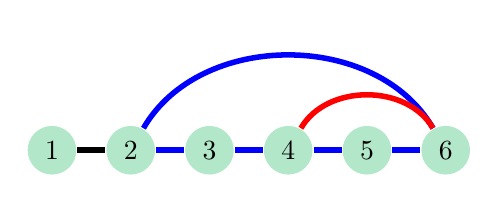
\begin{tikzpicture}
            [scale=1,auto=left,thick,every node/.style={circle,fill=blue!30!green!30}]
            \node (1) at (0,0) {1};
            \node (2) at (1,0) {2};
            \node (3) at (2,0) {3};
            \node (4) at (3,0) {4};
            \node (5) at (4,0) {5};
            \node (6) at (5,0) {6};
            \draw[line width=2pt] (1) -- (2);
            \draw[line width=2pt, blue] (2) -- (3);
            \draw[line width=2pt, blue] (3) -- (4);
            \draw[line width=2pt ,blue] (4) -- (5);
            \draw[line width=2pt, blue] (5) -- (6);
            \draw[line width=2pt, blue] (6) to[bend right=60] (2);
            \draw[line width=2pt, red] (6) to[bend right=60] (4);
        \end{tikzpicture}
    \end{minipage}\hfill
    \begin{minipage}{0.48\textwidth}
        \centering
        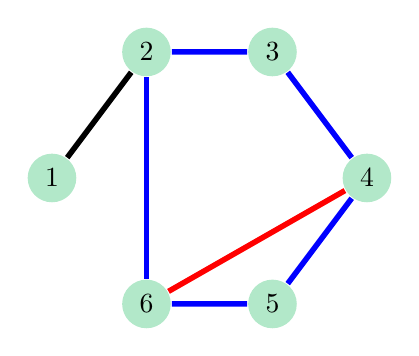
\begin{tikzpicture}
            [scale=.8,auto=left,thick,every node/.style={circle,fill=blue!30!green!30}]
            \node (1) at (-2.5, 0) {1};
            \node (2) at (-1, 2) {2};
            \node (3) at ( 1, 2) {3};
            \node (4) at ( 2.5, 0) {4};
            \node (5) at ( 1,-2) {5};
            \node (6) at (-1,-2) {6};
            \draw[line width=2pt] (1) -- (2);
            \draw[line width=2pt, blue] (2) -- (3);
            \draw[line width=2pt, blue] (3) -- (4);
            \draw[line width=2pt ,blue] (4) -- (5);
            \draw[line width=2pt, blue] (5) -- (6);
            
            \draw[line width=2pt, blue] (2) -- (6);
            \draw[line width=2pt, red] (4) -- (6);

        \end{tikzpicture}
    \end{minipage}
    \caption{An example walk following the procedure to find a cycle with a chord in a graph of minimum degree at least 3. The cycle and chord found by the procedure are marked by blue and red respectively. Note that this example includes only vertices and edges visited and traversed by the procedure.}
    \label{fig:Q6}
\end{figure}

\section*{A Planarity Algorithm}

\subsection*{Question 7}
We now consider the following algorithm for determining if a graph is planar or not.

\subsubsection*{The algorithm}
\begin{enumerate}
    \item Find the core $G^*$ of $G$
    \item If $G^*$ is empty, $G$ is planar
    \item Else find a cycle $C$ in $G^*$ with a chord $e$.
    \item Find the bridges of $C$ in $G^*$ and the interleave graph $H$.
    \item If $H$ is not bipartite then $G$ is not planar.
    \item Else $G$ is planar if and only if $G^*-e$ is planar.
\end{enumerate}

\subsubsection*{Explanation of algorithm}
We explain each step as follows:
\begin{enumerate}
    \item 
    Since none of the operations involved in finding the core of a graph affect planarity we have that $G$ is planar if and only if $G^*$ is planar. We therefore choose to simplify the problem and consider only the core.
    \item
    An empty graph is clearly planar and so if $G^*$ is the empty graph it follows that $G$ is planar.
    \item
    By construction of the core all vertices in $G^*$ are either of degree 0 or of degree at least 3. Therefore, by the procedure described in Question 6 we can find a cycle $C$ with a chord $e$ in $G^*$.
    \item
    We can then find the bridges of the cycle $C$ and the interleave graph $H$.
    \item
    A result from Question 3 was that a graph is planar if and only if its interleave graph is planar. Taking the negation of this result we conclude that $H$ is not bipartite implies $G$ is not planar.
    \item
    Removing chord $e$ does not affect the planarity of the graph because we have that $H$ is bipartite which means that $G^*$ can be drawn without any edges crossing between bridges. Chord $e$ is a bridge and is itself clearly planar so we can remove it without affecting planarity to simplify the problem.
\end{enumerate}

Finally, we observe that the algorithm must terminate: Every loop, at step 6, an edge is removed making $e(G^*)$ a strictly decreasing function of the number of iterations. The algorithm cannot loop forever since $G$ is finite, if the algorithm loops sufficiently then $e(G^*)$ will eventually reach 0 at which point the algorithm will definitely terminate at step 2. A simple bound for the maximum iterations required would be
\[ max(e(G)) = {|G|\choose2} \].

\subsection*{Question 8}

Script is\_planar.m (pg.\pageref{Pis_planar}) implements this algorithm to determine whether a given graph is planar. Script q8.m (pg.\pageref{PQ8}) is a short script for assisting in testing is\_planar.m. Script is\_planar correctly identifies all the platonic solid graphs (from Question 1) as planar. It also correctly identifies slight variations of the platonic solids including correctly identifying the graphs included in figure \ref{fig:q8}.

\begin{figure}[H]
    \centering
    \begin{minipage}{0.48\textwidth}
        \centering
        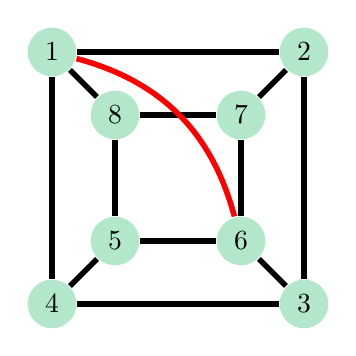
\begin{tikzpicture}
            [scale=.8,auto=left,thick,every node/.style={circle,fill=blue!30!green!30}]
            \node (1) at (-2,2) {1};
            \node (2) at (2,2) {2};
            \node (3) at (2,-2) {3};
            \node (4) at (-2,-2) {4};
            \node (5) at (-1,-1) {5};
            \node (6) at (1,-1) {6};
            \node (7) at (1,1) {7};
            \node (8) at (-1,1) {8};
            %
            \draw[line width=2pt] (1) -- (2);
            \draw[line width=2pt] (2) -- (3);
            \draw[line width=2pt] (3) -- (4);
            \draw[line width=2pt] (4) -- (1);
            \draw[line width=2pt] (1) -- (8);
            \draw[line width=2pt] (2) -- (7);
            \draw[line width=2pt] (3) -- (6);
            \draw[line width=2pt] (4) -- (5);
            \draw[line width=2pt] (5) -- (6);
            \draw[line width=2pt] (6) -- (7);
            \draw[line width=2pt] (7) -- (8);
            \draw[line width=2pt] (8) -- (5);
            %
            \draw[line width=2pt, red] (1) to[bend left=30] (6);
        \end{tikzpicture}
    \end{minipage}\hfill
    \begin{minipage}{0.48\textwidth}
        \centering
        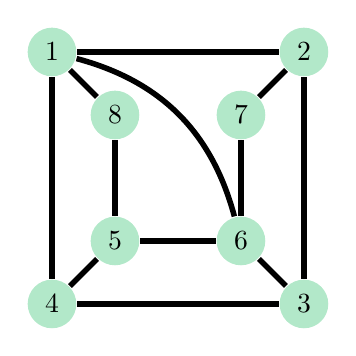
\begin{tikzpicture}
            [scale=.8,auto=left,thick,every node/.style={circle,fill=blue!30!green!30}]
            \node (1) at (-2,2) {1};
            \node (2) at (2,2) {2};
            \node (3) at (2,-2) {3};
            \node (4) at (-2,-2) {4};
            \node (5) at (-1,-1) {5};
            \node (6) at (1,-1) {6};
            \node (7) at (1,1) {7};
            \node (8) at (-1,1) {8};
            %
            \draw[line width=2pt] (1) -- (2);
            \draw[line width=2pt] (2) -- (3);
            \draw[line width=2pt] (3) -- (4);
            \draw[line width=2pt] (4) -- (1);
            \draw[line width=2pt] (1) -- (8);
            \draw[line width=2pt] (2) -- (7);
            \draw[line width=2pt] (3) -- (6);
            \draw[line width=2pt] (4) -- (5);
            \draw[line width=2pt] (5) -- (6);
            \draw[line width=2pt] (6) -- (7);
            %\draw[line width=2pt] (7) -- (8);
            \draw[line width=2pt] (8) -- (5);
            %
            \draw[line width=2pt] (1) to[bend left=30] (6);
        \end{tikzpicture}
    \end{minipage}
    \caption{Two variations of II-17-7-Platonic\_6.txt. Left a non-planar variation. Right: a planar variation.}
    \label{fig:q8}
\end{figure}

\subsection*{Question 9}

Script max\_planar.m (pg.\pageref{Pmax_planar}) builds a random maximal planar graph of specified $n$ vertices. It starts with an empty graph and adds each of the possible edges in a random order, keeping only those edges which don't violate planarity. It returns a graph as an edge list and also includes the number of edges added before the first violation of planarity. Figure \ref{fig:Q9ex} includes an example application of this script.

\begin{figure}[H]
    \centering
    \begin{minipage}{0.48\textwidth}
        \centering
        \begin{verbatim}
>> [graph,beforeViolation] = max_planar(5)

graph =

     2     5
     1     3
     4     5
     2     3
     3     5
     1     2
     1     5
     3     4
     2     4

beforeViolation =

     9
        \end{verbatim}
    \end{minipage}\hfill
    \begin{minipage}{0.48\textwidth}
        \centering
        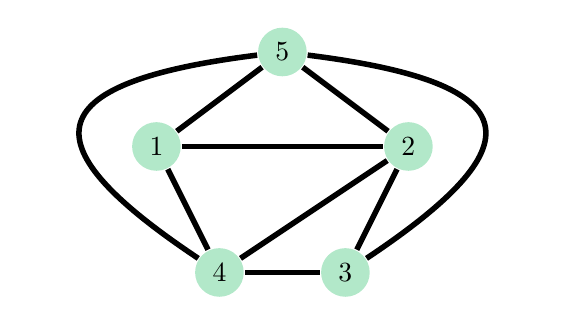
\begin{tikzpicture}
            [scale=.8,auto=left,thick,every node/.style={circle,fill=blue!30!green!30}]
            \node (5) at (0, 3.5) {5};
            \node (2) at (2, 2) {2};
            \node (3) at (1, 0) {3};
            \node (4) at (-1, 0) {4};
            \node (1) at (-2,2) {1};
            \draw[line width=2pt] (5) .. controls (-4, 3) and (-4, 2)  .. (4);
            \draw[line width=2pt] (2) -- (5);
            \draw[line width=2pt] (3) -- (4);
            \draw[line width=2pt] (2) -- (4);
            \draw[line width=2pt] (1) -- (2);
            \draw[line width=2pt] (5) .. controls (4, 3) and (4, 2)  .. (3);
            \draw[line width=2pt] (2) -- (3);
            \draw[line width=2pt] (1) -- (5);
            \draw[line width=2pt] (1) -- (4);

        \end{tikzpicture}
    \end{minipage}
    \caption{An example random maximal planar graph of size 5 generated by max\_planar.m}
    \label{fig:Q9ex}
\end{figure}

\subsubsection*{Edges of a maximal planar graph}
The maximum number of edges that a planar graph of $n$ vertices can have is $3n-6$.

\bigskip 
To prove this we start with Euler's formula which states that for a graph $G$ with $|G|=n\geq1$ and $e(G)=m$ that can be drawn with $l$ faces then:
\[ n-m+l=2 \]

Next we make the following two observations about drawings:
\begin{itemize}
    \item Each edge boarders at most 2 faces
    \item Each face boarders at most 3 edges
\end{itemize}
Combining these two observations we deduce:
\[ 3l \leq 2m \]
Substituting this inequality into Euler's formula we reach the following:
\begin{align*}
    n-m+l &= 2 \\
    n-m+\frac{2m}{3} &\geq 2 \\
    3n-m &\geq 6 \\
    m &\leq 3n-6
\end{align*}
Therefore a planar graph may have no more than $3n-6$ edges. We now demonstrate that a planar graph may attain this limit by giving an example method for constructing such a graph. For $G$ with $n$ vertices we draw as follows:
\begin{itemize}
    \item Draw an $n$-gon. This contains $n$ edges.
    \item Triangulate the inside of the $n$-gon. That is, add edges within the n-gon such that the only faces within the $n$-gon are triangles. One way to do this is to choose a vertex and connect the chosen vertex to every other vertex in the $n$-gon. This adds $n-3$ edges.
    \item Triangulate the outside of the $n$-gon. This can be done similarly to above, however, at this step we must avoid drawing edges that are already present within the $n$-gon for a second time. We can actually use the same method for triangulation as above except that the vertex chosen cannot be the same as in the previous step. This adds $n-3$ edges.
    \item Now all faces of the drawing at triangles and so it is impossible to add a further edge without compromising planarity.
\end{itemize}
Adding up the edges of the drawing: $n + (n-3) + (n-3) = 3n-6$ (Figure \ref{fig:Q9a} includes a planar graph of 6 vertices drawn according to this method). Therefore, by showing the bound is attainable we achieve the desired result.

\begin{figure}[H]
    \centering
    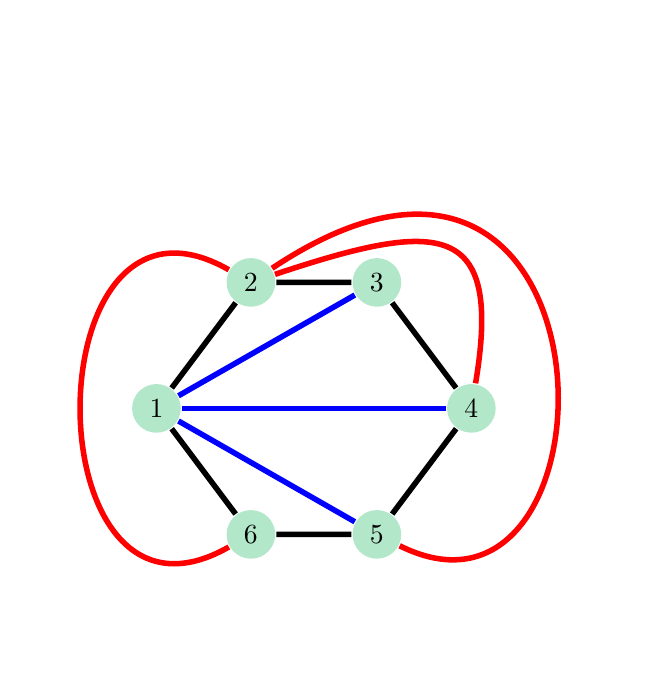
\begin{tikzpicture}
        [scale=.8,auto=left,thick,every node/.style={circle,fill=blue!30!green!30}]
        \node (1) at (-2.5, 0) {1};
        \node (2) at (-1, 2) {2};
        \node (3) at ( 1, 2) {3};
        \node (4) at ( 2.5, 0) {4};
        \node (5) at ( 1,-2) {5};
        \node (6) at (-1,-2) {6};
        
        % the circle
        \draw[line width=2pt] (1) -- (2);
        \draw[line width=2pt] (2) -- (3);
        \draw[line width=2pt] (3) -- (4);
        \draw[line width=2pt] (4) -- (5);
        \draw[line width=2pt] (5) -- (6);
        \draw[line width=2pt] (6) -- (1);
        % inside the circle
        \draw[blue, line width=2pt] (1) -- (3);
        \draw[blue, line width=2pt] (1) -- (4);
        \draw[blue, line width=2pt] (1) -- (5);
        % outside the circle
        \draw[red, line width=2pt] (2) .. controls (2, 3) and (3,3) .. (4);
        \draw[red, line width=2pt] (2) .. controls (5,6) and (5, -4) .. (5);
        \draw[red, line width=2pt] (2) .. controls (-4.5,4) and (-4.5, -4) .. (6);
    \end{tikzpicture}
    \caption{A drawing of a maximal planar graph for the case $n=6$. The colours highlight the construction of the drawing. Black: lines from the original hexagon drawn. Blue/red: lines from triangulation of vertices inside/outside the hexagon.}
    \label{fig:Q9a}
\end{figure}

\subsubsection*{Generating maximal planar graphs of 40 vertices}

Script Q9.m (pg.\pageref{PQ9}) generates 20 maximal planar graphs with 40 vertices using the max\_planar.m function. Figure \ref{fig:Q9b} includes the output from a running of Q9.m, the graphs are returned as edge lists but in the output are printed in shorthand for brevity. Inspecting the number of edges in each graph (eg. \texttt{[112x2 double]} is a graph of 112 edges) we note that none of the graphs exceed the maximum number of edges, $3n-6=3\times40-6=114$, in accordance with the previous result. Interestingly, we note that a large proportion (50\%) of the graphs actually attain this maximum and all others are within a relatively small amount (at most 4 edges) of this maximum.

\begin{figure}
    \centering
    \begin{verbatim}
graphs =

  20×2 cell array

    [112×2 double]    [38]
    [111×2 double]    [40]
    [114×2 double]    [32]
    [114×2 double]    [40]
    [113×2 double]    [41]
    [114×2 double]    [39]
    [113×2 double]    [51]
    [113×2 double]    [43]
    [114×2 double]    [35]
    [114×2 double]    [40]
    [114×2 double]    [40]
    [114×2 double]    [46]
    [114×2 double]    [33]
    [113×2 double]    [40]
    [110×2 double]    [38]
    [113×2 double]    [48]
    [113×2 double]    [43]
    [114×2 double]    [42]
    [114×2 double]    [48]
    [113×2 double]    [39]
    
averageEdgesBeforeViolation =

   40.8000
    \end{verbatim}
    \caption{Output from script Q9.m. Each row represents a graph. The first element is the edge list (note MATLAB prints this out as short hand here but all edge lists are stored in full by the script). The second element is the number of edges added before the first violation of planarity in the construction. Then \texttt{averageEdgesBeforeViolation} is the average edges added before the first violation is included at.}
    \label{fig:Q9b}
\end{figure}

\subsubsection*{Edges before first violation}
Figure \ref{fig:Q9b} also includes the number of edges added before the first violation of planarity for each graph and an average of these values. Interestingly this average is $40.8$ which is approximately the number of vertices, $n=40$.

\subsubsection*{Drawing of a 40 vertex maximal planar graph}

We can inspect the graphs constructed by Q9.m and use the script, tutte.m, from Question 1 to draw them. As an example we do this for one of the 20 graphs generated above. However, in order to apply Tutte's algorithm we first require a cycle with only one bridge. Maximal planar graphs are fully triangulated (all faces are triangles), if not all faces are triangles then for any face of more than 3 sides there is at least one edge yet to be drawn which can be added across the face. Now we observe that every triangle in a maximal planar graph is a cycle with a single bridge which includes all other vertices and edges. So to apply Tutte's algorithm we need to simply identify one of these many triangles, script find\_triangle.m (pg.\pageref{Pfind_triangle} is a small function to do this. We can now draw a graph.

\bigskip
Figure \ref{fig:Q9plot_full} is a drawing generated by tutte.m with a cycle identified by find\_triangle.m. See figures \ref{fig:Q9plot_detail0} - \ref{fig:Q9plot_detail3} for enlargements of the denser areas of the drawing showing that this drawing is indeed planar.

\begin{figure}[H]
    \centering
    \includegraphics[width=0.98\columnwidth]{Q9_full_crop.png}
    \caption{A planar drawing of a maximal planar graph generated by Q9.m plotted using the tutte.m script from Question 1. See figures \ref{fig:Q9plot_detail0} - \ref{fig:Q9plot_detail3} for enlargements to make clear the denser ares of the graph.}
    \label{fig:Q9plot_full}
\end{figure}

\begin{figure}[H]
    \centering
    \includegraphics[width=0.6\columnwidth]{Q9zoom_in0_crop.png}
    \caption{See figure \ref{fig:Q9plot_detail0} for an enlargement of the highlighted portion of this figure.}
    \label{fig:Q9plot_detail0}
\end{figure}
\begin{figure}[H]
    \centering
    \includegraphics[width=0.9\columnwidth]{Q9zoom_in1_crop.png}
    \caption{An enlargement of figure \ref{fig:Q9plot_detail0}. See figure \ref{fig:Q9plot_detail2} for an enlargement of the highlighted portion of this figure.}
    \label{fig:Q9plot_detail1}
\end{figure}
\begin{figure}[H]
    \centering
    \includegraphics[width=0.95\columnwidth]{Q9zoom_in2_crop.png}
    \caption{An enlargement of figure \ref{fig:Q9plot_detail1}. See figure \ref{fig:Q9plot_detail3} for an enlargement of the highlighted portion of this figure.}
    \label{fig:Q9plot_detail2}
\end{figure}
\begin{figure}[H]
    \centering
    \includegraphics[width=0.7\columnwidth]{Q9zoom_in3_crop.png}
    \caption{An enlargement of figure \ref{fig:Q9plot_detail2}.}
    \label{fig:Q9plot_detail3}
\end{figure}

\newpage
\subsection*{Question 10: Complexity}

We now estimate the complexity of the algorithm discussed in Question 8. Firstly we note that the number of iterations the algorithm could experience is $O(m)$ because each loop the graph looses at lease one edge (in step 6). Next we must consider the complexity of each subroutine involved in the algorithm:

\begin{itemize}
    \item 
    \subsubsection*{Finding the core of a graph (find\_core.m)}
    For this method the worst case is the scenario in which the core is the empty graph but to reach this we must iterate $m$ times on $G$, every time checking every edge still present. This gives a complexity of $O(n(n-1)/2 = O(n^2)$.
    \item
    \subsubsection*{Finding a cycle in $G^*$ with a chord $e$ (find\_cycle\_with\_chord.m)}
    For this method the worst case is a scenario in which the walk involves travelling a path of maximal length which can be at most $n$. At each step, the current vertex's neighbourhood is compared with the route so far. Therefore we estimate a complexity of $O(n^2)$.
    \item
    \subsubsection*{Finding the bridges of $C$ in $G^*$ (find\_bridges.m)}
    This method involves visiting every vertex of $G^*$ once, once assigned to a component it is ignored. This gives a complexity of $O(n)$.
    \item
    \subsubsection*{Finding the interleave graph $H$ (find\_interleave.m)}
    This worst scenario for this method is one in which the number of bridges is maximised. A bridge requires at least one edge, therefore the maximum number of bridges is $O(m)$. Comparing bridges is order $O(n)$ as it involves comparing anchor points with the cycle. Overall, we therefore estimate a total complexity of $O(mn)$.
    \item
    \subsubsection*{Checking if $H$ is bipartite (is\_bipartite.m)}
    This method involves colouring vertices until we find a contradiction or successfully partition the whole graph. Therefore the worst case involves finding no contradictions and so needing to partition the entire graph, this is $O(n)$. In order to colour a given vertex we must compare it with already coloured vertices, this is $O(n)$. Overall, therefore, we estimate a complexity of $O(n^2)$.
\end{itemize}

Overall, combining the above estimates we reach the following estimate for the complexity of the algorithm:
\[ O(m) \times [O(n^2) + O(n^2) + O(n) + O(mn) + O(n^2)] = O(m^2n+mn^2)) \]


\pagebreak
\section*{Programs}

\subsection*{Q1.m}\label{PQ1}
Dependencies: tutte.m
\lstinputlisting{Q1.m}

\subsection*{tutte.m}\label{Ptutte}
Dependencies: edgList\_to\_adjList.m, adjList\_to\_adjMat.m
\lstinputlisting{tutte.m}

\subsection*{edgList\_to\_adjList.m}\label{PedgList_to_adjList}
\lstinputlisting{edgList_to_adjList.m}

\subsection*{adjList\_to\_adjMat.m}\label{PadjList_to_adjMat}
\lstinputlisting{adjList_to_adjMat.m}

\subsection*{K2\_P5.txt}\label{K2_P5}
\lstinputlisting{K2_P5.txt}

\subsection*{find\_comp.m}\label{Pfind_comp}
\lstinputlisting{find_comp.m}

\subsection*{find\_bridges.m}\label{Pfind_bridges}
Dependencies: edgList\_to\_adjList.m, find\_comp.m
\lstinputlisting{find_bridges.m}

\newpage
\subsection*{find\_interleave.m}\label{Pfind_interleave}
\lstinputlisting{find_interleave.m}

\newpage
\subsection*{is\_bipartite.m}\label{Pis_bipartite}
Dependencies: edgList\_to\_adjList.m
\lstinputlisting{is_bipartite.m}

\newpage
\subsection*{find\_core.m}\label{Pfind_core}
Dependencies: edgList\_to\_adjList.m, add\_edges.m, remove\_edges.m
\lstinputlisting{find_core.m}

\subsection*{add\_edges.m}\label{Padd_edges}
\lstinputlisting{add_edges.m}

\subsection*{remove\_edges.m}\label{Premove_edges}
\lstinputlisting{remove_edges.m}

\newpage
\subsection*{find\_cycle\_with\_chord.m}\label{Pfind_cycle_with_chord}
Dependencies: edgList\_to\_adjList.m
\lstinputlisting{find_cycle_with_chord.m}

\subsection*{is\_planar.m}\label{Pis_planar}
Dependencies: find\_core.m, find\_cycle\_with\_chord.m, find\_bridges.m, \newline
              find\_interleave.m, is\_bipartite.m
\lstinputlisting{is_planar.m}

\newpage
\subsection*{Q8.m}\label{PQ8}
Dependencies: is\_planar.m, add\_edges.m, remove\_edges.m
\lstinputlisting{Q8.m}

\subsection*{max\_planar.m}\label{Pmax_planar}
Dependencies: is\_planar.m
\lstinputlisting{max_planar.m}

\newpage
\subsection*{Q9.m}\label{PQ9}
Dependencies: max\_planar.m
\lstinputlisting{Q9.m}

\subsection*{find\_triangle.m}\label{Pfind_triangle}
Dependencies: edgList\_to\_adjList.m
\lstinputlisting{find_triangle.m}

\end{document}
